\documentclass[12pt]{article}

\usepackage{amsmath}
\usepackage[super]{nth}
\usepackage[utf8]{inputenc}
\usepackage[T1]{fontenc}
\usepackage{textcomp}
\usepackage{gensymb}
\usepackage{graphicx}
\usepackage{hyperref}
\usepackage{caption}
\usepackage{float}

\pagenumbering{arabic}

\begin{document}

\title{Graphical Analysis - Literature Study}
\date{December 06, 2016}
\author{Rafael De Smet}

\maketitle
\tableofcontents
\newpage
\section{Introduction}

In this paper I will be discussing several graphical analysis and text recognition algorithms. These algorithms will return data which are used to base the music generation on. Not all algorithms are used in the code, but are discussed for the sake of completeness.

\section{Image Processing Algorithms}

\subsection{Edge Detection}

The concept of edge detection is pretty straightforward. The algorithms try to detect all the edges in an image. Edges are the contours of objects and shapes in the image.
Edge detection algorithms all use what are called convolution kernels. A kernel in image processing is a small matrix used to apply effects to an image, such as blurring and outlining. Here we will see kernels used for edge detection only. Listed below are six of the best and most used algorithms.

\begin{itemize}
        \item Sobel 
        \item Frei-Chen
        \item Prewitt
        \item Roberts Cross
        \item LoG
        \item Scharr
\end{itemize}

\subsubsection{Convolution kernel}

Convolution is the technique of multiplying together two arrays of different size but of the same dimension. An array of dimension two simply is a matrix. When working with images the pixels are represented as a (2D) matrix and the kernel is also a 2D matrix.
The kernel is a small matrix that we will multiply with the image matrix to perform the convolution. This kernel matrix is different for each edge detection algorithm. We will see examples of different matrices later in this paper. 
\newline

The idea of these algorithms is to create a new image that shows the edges of the original image. Each pixel of the original image is added to its local neighbours, weighted by the kernel. This produces a new image. The result of the matrix multiplication results in new pixel values that denote the edges of the image. 
Mathematically we can write the convolution as follows, with $O$ the output image, $I$ the input image and $K$ the kernel. $I(i,j)$ means the pixel on the $i^{th}$ row and the $j^{th}$ column.

\begin{equation}
O(i, j) =  \sum\limits_{k=1}^m\sum\limits_{l=1}^n I(i + k - 1, j + l - 1)K(k,l)
\end{equation}
\newline

An example will clarify the previous.

\begin{figure}[h]
\centering
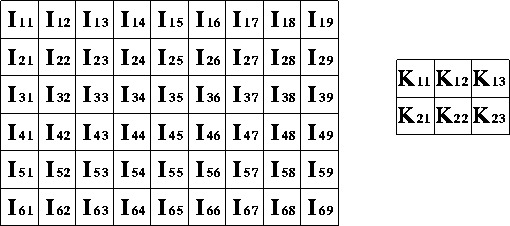
\includegraphics[scale = 0.5]{img/convolution}
\caption{A pixel matrix and a kernel matrix}
\label{kernel}
\end{figure}

Using the kernel matrix we will compute every new pixel of the output image, by sliding the kernel matrix over the original pixels. Each kernel position corresponds to a single output pixel, the value of which is calculated by equation (1).
\newline

In our example, the value of the bottom right pixel in the output image will be found as follows [2]:

\begin{equation}
O_{57} = I_{57}K_{11} + I_{58}K_{12} + I_{59}K_{13} + I_{67}K_{21} + I_{68}K_{22} + I_{69}K_{23}
\end{equation}
\newpage

In figure \ref{picasso} you can see a painting by Picasso. We will use this image to see how well the different edge detection algorithms work.

\begin{figure}[h]
\centering
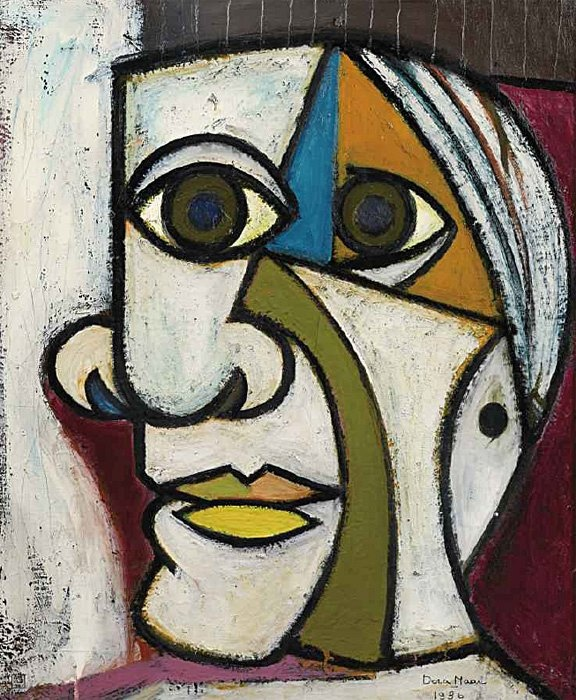
\includegraphics[scale = 0.39]{img/picasso}
\caption{Picasso}
\label{picasso}
\end{figure}

\subsubsection{Sobel}

 The Sobel algorithm performs a 2D spatial gradient measurement and defines regions of 'high spatial frequency' or edges. It uses two 3x3 kernels, one for the horizontal edges and one for the vertical edges. These two kernels are applied consecutively and the results are combined to define all the edges. In figure \ref{sobel} you can see the result of the Sobel filter.
 \newline

 The horizontal kernel: 
 $\begin{vmatrix}
        -1 & 0 & +1\\
        -2 & 0 & +2\\
        -1 & 0 & +1\\
\end{vmatrix}$
and the vertical kernel:
$\begin{vmatrix}
        +1 & +2 & +1\\
        0 & 0 & 0\\
        -1 & -2 & -1\\
\end{vmatrix}$

\begin{figure}[h]
\centering
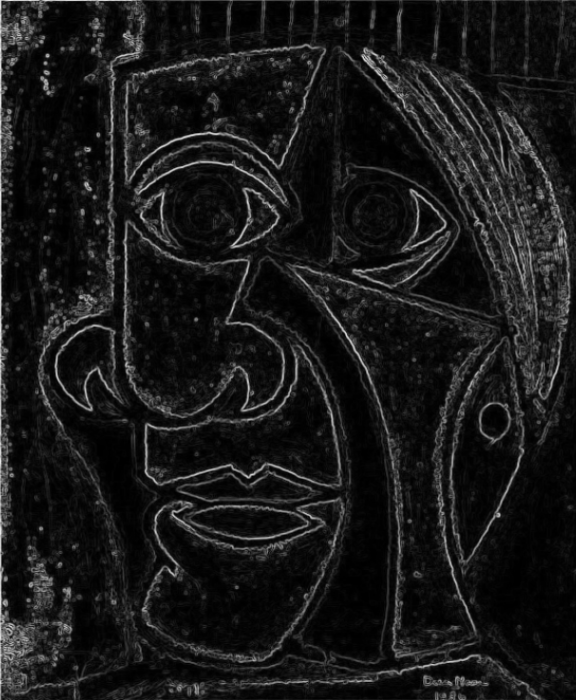
\includegraphics[scale = 0.39]{img/picassoSobel}
\caption{Sobel filter applied to figure \ref{picasso}}
\label{sobel}
\end{figure}
\newpage

\subsubsection{Frei-Chen}
 The Frei-Chen algorithm also uses 3x3 kernels, but this time there are nine different convolution kernels. The four first matrices, G1, G2, G3, G4, are used for edges, the next four are used for lines and $G_9$ is used to compute averages. $G_9$ attenuates the impact of the computations from the other matrices. Figure \ref{freichen} shows the result of the Frei-Chen filter.
\newline
\newline
 $G_1$ = $\frac{1}{2\sqrt2}$ $\begin{vmatrix}
        1 & \sqrt2 & 1\\
        0 & 0 & 0\\
        -1 & -\sqrt2 & -1\\
\end{vmatrix}$\hspace{5mm}
$G_2$ = $\frac{1}{2\sqrt2}$$\begin{vmatrix}
        1 & 0 & -1\\
        \sqrt2 & 0 & -\sqrt2\\
        1 & 0 & -1\\
\end{vmatrix}$\hspace{5mm}
$G_3$ = $\frac{1}{2\sqrt2}$$\begin{vmatrix}
        0 & -1 & \sqrt2\\
        1 & 0 & -1\\
        -\sqrt2 & 1 & 0\\
\end{vmatrix}$\hspace{5mm}
\newline
$G_4$ = $\frac{1}{2\sqrt2}$$\begin{vmatrix}
        \sqrt2 & -1 & 0\\
        -1 & 0 & 1\\
        0 & 1 & -\sqrt2\\
\end{vmatrix}$\hspace{5mm}
$G_5$ = $\frac{1}{2}$$\begin{vmatrix}
        0 & 1 & 0\\
        -1 & 0 & -1\\
        0 & 1 & 0\\
\end{vmatrix}$\hspace{10mm}
$G_6$ = $\frac{1}{2}$$\begin{vmatrix}
        -1 & 0 & 1\\
        0 & 0 & 0\\
        1 & 0 & -1\\
\end{vmatrix}$\hspace{5mm}
\newline
$G_7$ = $\frac{1}{6}$$\begin{vmatrix}
        1 & -2 & 1\\
        -2 & 4 & -2\\
        1 & -2 & 1\\
\end{vmatrix}$\hspace{13mm}
$G_8$ = $\frac{1}{6}$$\begin{vmatrix}
        -2 & 1 & -2\\
        1 & 4 & 1\\
        -2 & 1 & -2\\
\end{vmatrix}$\hspace{11mm}
$G_9$ = $\frac{1}{3}$$\begin{vmatrix}
        1 & 1 & 1\\
        1 & 1 & 1\\
        1 & 1 & 1\\
\end{vmatrix}$\hspace{5mm}

\begin{figure}[h]
\centering
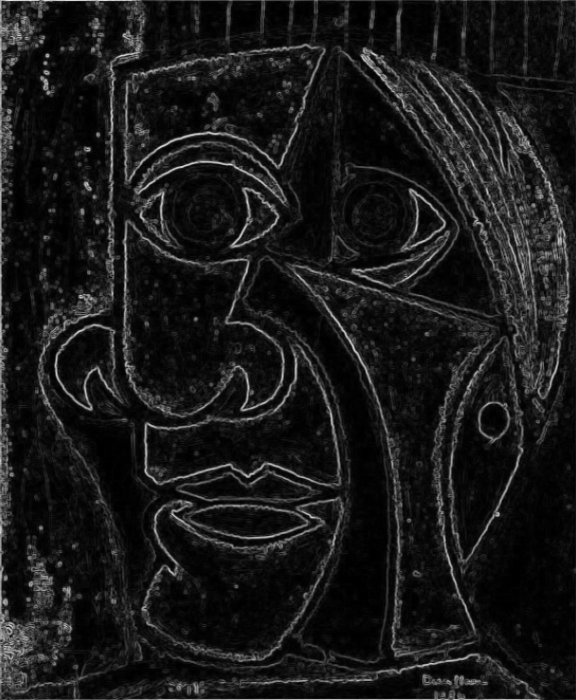
\includegraphics[scale = 0.39]{img/picassoFreiChen}
\caption{Frei-Chen filter applied to figure \ref{picasso}}
\label{freichen}
\end{figure}

\subsubsection{Prewitt}
This algorithm is very similar to the Sobel algorithm. Again, two kernels are used, one for the horizontal and one for the vertical edges. In this case the kernels are basic convolution filters of the following form. 
\newline

Horizontal filter = $\begin{vmatrix}
        1 & 1 & 1\\
        0 & 0 & 0\\
        -1 & -1 & -1\\
\end{vmatrix}$\hspace{11mm}
Vertical filter = $\begin{vmatrix}
        -1 & 0 & 1\\
        -1 & 0 & 1\\
        -1 & 0 & 1\\
\end{vmatrix}$
\newline

\begin{figure}[h]
\centering
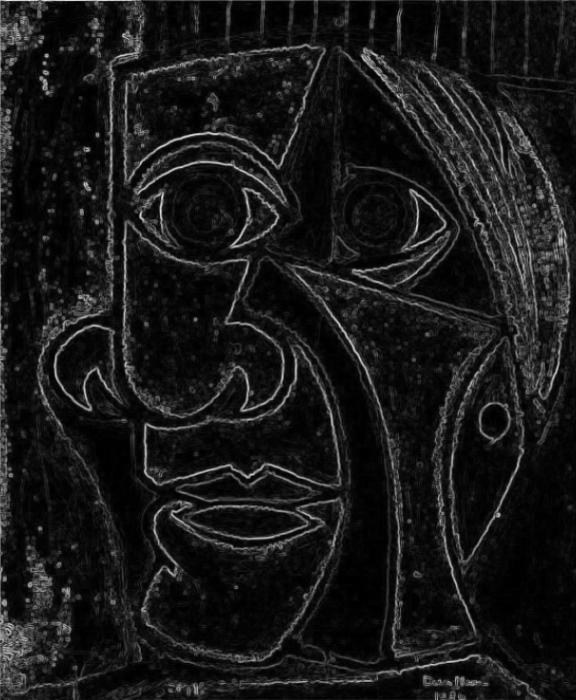
\includegraphics[scale = 0.39]{img/picassoPrewitt}
\caption{Prewitt filter applied to figure \ref{picasso}}
\label{prewitt}
\end{figure}
\newpage

\subsubsection{Roberts Cross}
This algorithm uses even simpler kernels than Prewitt does. This time we use two 2x2 kernels. These kernels correspond to the edges running at 45° to the pixel grid, one for each of the two perpendicular orientations. Figure \ref{robertscross} shows the result of the Roberts Cross filter.
\newline

Horizontal filter = $\begin{vmatrix}
        1 & 0 \\
        0 & -1 \\
\end{vmatrix}$\hspace{11mm}
Vertical filter = $\begin{vmatrix}
        0 & 1\\
        -1 & 0\\
\end{vmatrix}$

\begin{figure}[h]
\centering
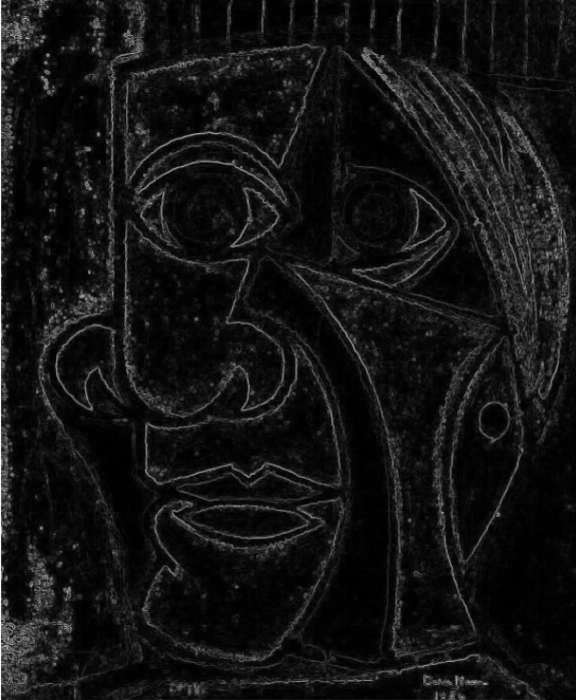
\includegraphics[scale = 0.39]{img/picassoRobertsCross}
\caption{Roberts Cross filter applied to figure \ref{picasso}}
\label{robertscross}
\end{figure}

\subsubsection{LoG}
This algorithm first applies Gaussian filtering\footnote{The Gaussian filter is used to blur images and remove noise and detail.} to the image and then the Laplacian method for edge detection\footnote{The Laplacian method highlights regions in the image of rapid intensity change, so it is useful for edge detection.}, hence the name "Laplacian of Gaussian" (LoG).
The edge points of an image are detected by finding the zero crossings of the \nth{2} derivative of the image intensity. Because the \nth{2} derivative is very sensitive to noise, which could give us bad results, the Gaussian filter is used to clear the noise from the image. In figure \ref{log}, you can find the result of this filter.
\newline

The R library OpenImageR\footnote{https://cran.r-project.org/web/packages/OpenImageR/OpenImageR.pdf} uses the following LoG mask.
\newline

LoG mask = $\begin{vmatrix}
        1 & 1 & 1\\
        1 & -8 & 1\\
        1 & 1 & 1\\
\end{vmatrix}$

\begin{figure}[h]
\centering
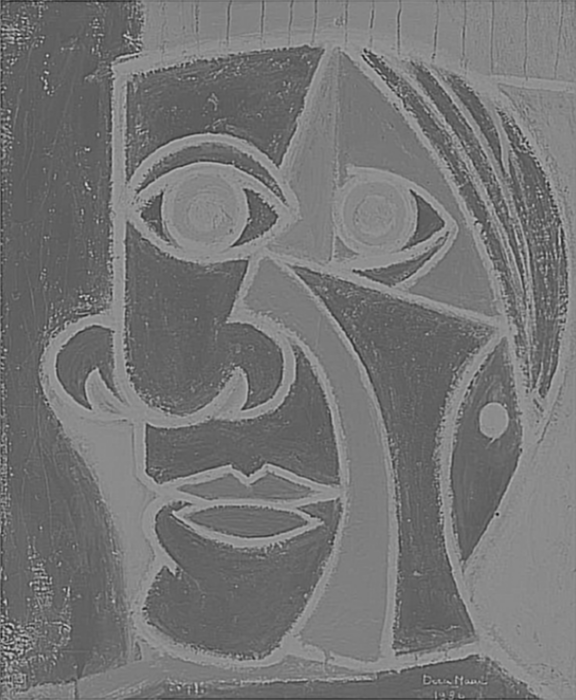
\includegraphics[scale = 0.39]{img/picassoLoG}
\caption{LoG filter applied to figure \ref{picasso}}
\label{log}
\end{figure}

\subsubsection{Scharr}
The last algorithm is again an extension of the Sobel algorithm. This operator improves rotational invariance, which means that if the image is rotated, the operator should define the same edges. Sobel can have difficulties with this aspect. There are many Scharr kernels, some even 5x5, but the following are most frequently used. Figure \ref{scharr} shows the results.
\newline

Horizontal filter = $\begin{vmatrix}
        3 & 10 & 3\\
        0 & 0 & 0\\
        -3 & -10 & -3\\
\end{vmatrix}$\hspace{11mm}
Vertical filter = $\begin{vmatrix}
        3 & 0 & -3\\
        10 & 0 & -10\\
        3 & 0 & -3\\
\end{vmatrix}$\hspace{5mm}

\begin{figure}[h]
\centering
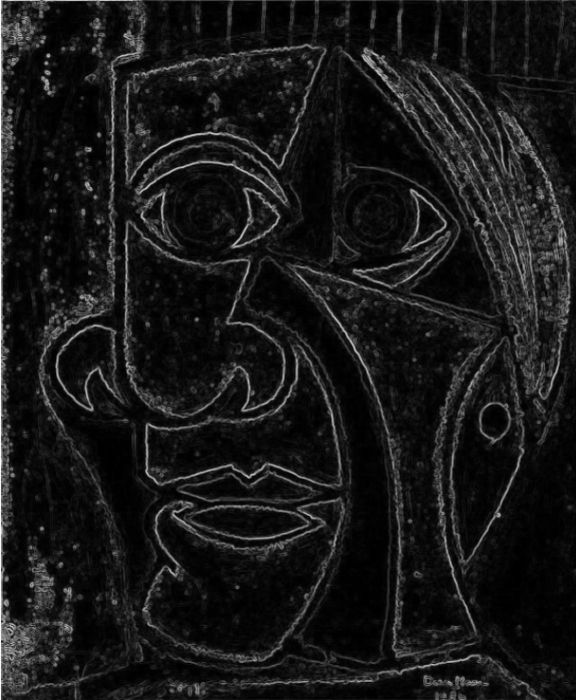
\includegraphics[scale = 0.39]{img/picassoScharr}
\caption{Scharr filter applied to figure \ref{picasso}}
\label{scharr}
\end{figure}
\newpage

\subsection{Noise Removal}

Every edge detection algorithm was based on a specific filter. Using this same idea of applying filters to images we can detect and remove typical noise, such as additive 'salt and pepper' and Gaussian noise. Analogous to the previous section, I will discuss several noise removal algorithms and the filters used. The first image of figure \ref{noise_original} is the image I will be using to discuss the results of the algorithms [14].
\newline

In this section I will be discussing the effects of the filters on two kinds of noise. In order to show the effects, I added two types of noises to the source image. The first is the 'salt and pepper' noise, the second image of figure \ref{noise_original}. 'Salt and pepper' noise can be seen as sparsely occuring white and black pixels on the image. This means that some pixel values are maximized (white) and some are minimized (black). The second is the Gaussian noise, which can be seen in the third image in figure \ref{noise_original}. Gaussian noise is statistical noise, which means the values it can take are Gaussian-distributed.

\begin{figure}[h]
\hspace*{-0.8cm}
\centering
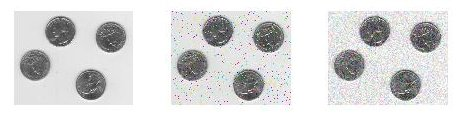
\includegraphics[scale = 1]{img/noise_orig}
\caption{Original image, 'salt and pepper' noise, Gaussian noise}
\label{noise_original}
\end{figure}

\subsubsection{Mean filtering}

This is the simplest linear filter and operates by giving weight $w_K$ to all the pixels in the neighbourhood of a certain pixel. Let's say we have a $N\times M$ neighbourhood, then we define the weight as follows: $w_K = \frac{1}{NM}$. The filter used in this technique is a $3\times3$ filter, as shown below.
\newline
\newline

Mean filter:
$\begin{bmatrix}
	0.1111 & 0.1111 & 0.1111 \\
	0.1111 & 0.1111 & 0.1111 \\
	0.1111 & 0.1111 & 0.1111 \\
\end{bmatrix}$
\newline
\newline

Figure \ref{noise_mean} shows the results of this filter. We can see that the filter is reasonably effective at removing the Gaussian noise (third image), but at the expense of losing detail in the edges of the image. The filter is not effective for the removal of the 'salt and pepper' noise. This is caused by a large deviation of the noise values from the typical values in the neighbourhood. This means that the average value is significantly influenced. This deviation is still very visible in the result.
\newline

The main disadvantages of mean filtering are (a) it is not robust to large noise deviations (also called outliers) and (b) the edges in the images will be blurred. This suggests we should look at a more robust (to statistical outliers) filter.

\begin{figure}[h]
\hspace*{-2cm}
\centering
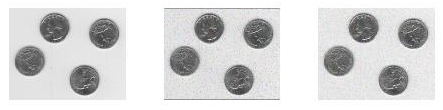
\includegraphics[scale = 1.2]{img/noise_mean}
\caption{Original image with mean filter, 'salt and pepper' noise with mean filter, Gaussian noise with mean filter}
\label{noise_mean}
\end{figure}

\subsubsection{Median filtering}

The mean filtering used the mean of a $N \times M$ neighbourhood as the weight. The median filtering uses the statistical median of the neighbourhood and is more suited because it preserves edges better while eliminating noise. Using the median is more robust to statistical outliers and does not create new unrealistic pixel values.
The disadvantage of this method is the high computational cost. To calculate the median of values, requires an ordering of those values.
\newline

In figure \ref{noise_median} you can see the results of this filter. It is clear that the median filter is very effective at removing the 'salt and pepper' noise. The removal of the Gaussian noise still is at the expense of a slight degradation in image quality. 

\begin{figure}[H]
\hspace*{-1.7cm}
\centering
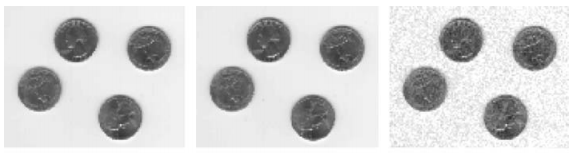
\includegraphics[scale = 0.9]{img/noise_median}
\caption{Original image with median filter, 'salt and pepper' noise with median filter, Gaussian noise with median filter}
\label{noise_median}
\end{figure}

\subsubsection{Rank filtering}

The median filter is nothing more than a special case of another filter type, the rank filter [14]. This filter follows four common steps.

\begin{itemize}
\item Define neighbourhood of the target pixel ($N\times N$).
\item Rank the pixels of the neighbourhood in ascending order.
\item Choose the rank pixel of the filter.
\item Set the filtered value to be equal to the value of the chosen rank pixel.
\end{itemize}

A common practice is to choose the minimum and maximum values of the pixels in the defined neighbourhood. Unsurprisingly, these filters are called minimum and maximum filters. In figure \ref{noise_rank} you can see the results. The effects on the 'salt and pepper' noise is not so good. Because it selects the maximum and minimun values, the high values in the image are amplified. The effects on the Gaussian noise are better. The noise is largely removed, but at the cost of image detail.

\begin{figure}[h]
\hspace*{-1.2cm}
\centering
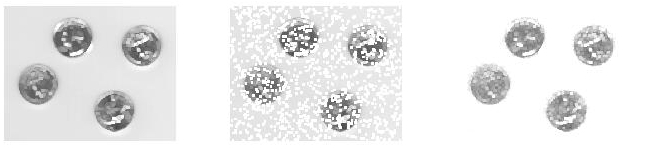
\includegraphics[scale = 0.8]{img/noise_rank}
\caption{Original image with rank filter, 'salt and pepper' noise with rank filter, Gaussian noise with rank filter}
\label{noise_rank}
\end{figure}
\newpage

\subsubsection{Gaussian filtering}

This technique differs from the other three I discussed. The filter used is a discrete kernel derived from the continuous 2D Gaussian function defined as follows [14]:

\begin{equation}
f(x,y) = \frac{1}{2\pi \sigma ^2} exp(-\frac{x^2 + y^2}{2\sigma^2})
\end{equation}
\newline

Applying the Gaussian filter has the effect of smoothing the image. The degree of smoothing is controlled by the choice of the standard deviation $\sigma$. The Fourier transform of the Gaussian function is a Gaussian function itself. This means that it is very convenient for the frequency-domain analysis of filters, but that discussion is out of scope for this paper.
\newline

In figure \ref{noise_gaussian} you can see the results. In all cases, the smoothing effect causes the edges to fade a little, but it also removes the noise to a certain degree. For this result I used a Gaussian filter with $\sigma = 2$. This filter gives the best result of all filters, with the median filter a close second choice.

\begin{figure}[h]
\hspace*{-1.2cm}
\centering
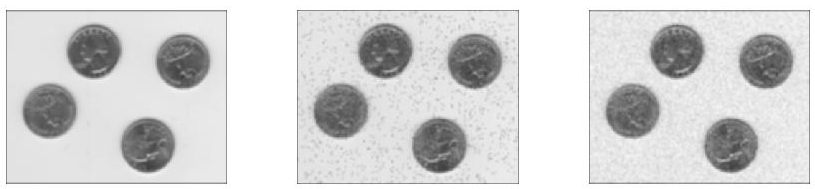
\includegraphics[scale = 0.6]{img/noise_gaussian}
\caption{Original image with Gaussian filter ($\sigma = 2$), 'salt and pepper' noise with Gaussian filter, Gaussian noise with Gaussian filter}
\label{noise_gaussian}
\end{figure}
\newpage

\subsection{Color Analysis}
Only edge detection algorithms are not sufficient to get enough data from the image to form a musical interpretation. We will need some form of color analysis as well. This section describes some algorithms and methods to obtain information about the colors of the image.

\subsubsection{RGB - HSV - CMYK}
To represent color on the computer the RGB representation is the most commonly used. Each pixel is described using three values, the amount of red (R), green (G) and blue (B). Using these values we can count how many pixels in the image are dominantly red, green or blue. When we're going to translate the image data into musical patterns, we can match each color to another kind of music (happy, sad, etc...)
\newline

HSV, sometimes called HSB, is another representation of a pixel. This time we use the hue (color, denoted by H), the saturation (S) and the brightness or value (B or V) to describe the pixel. Where the RGB model consists of three values indicating the amounts of a certain color each pixel has, the HSV model consists of three independent components to form a color. 
\newline

\paragraph{Hue} First we have the hue, which is the color. The color is represented using a circle with all the colors on it. The value of this component is the degrees of the angle we have to make on the circle to get this color.  

\paragraph{Saturation} The saturation indicates the fullness of the color. This value is expressed in a percentage, with 0\% a gray, flat color and 100\%  a full, rich color.

\paragraph {Value of Brightness} The value or brightness indicates the amount of light of the color and is also expressed in a percentage, 0\% is black and 100\% is white.

\begin{figure}[h]
\centering
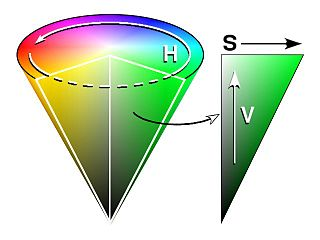
\includegraphics[scale = 0.45]{img/hsv}
\caption{The HSV color representation}
\label{hsv}
\end{figure}

CMYK is another representation of color, based on the mixing of four colors, cyan (C), magenta (M), yellow (Y) and key (K, black). This model is used frequently with printing, but not very interesting for this paper.

\subsubsection{Black And White Balance}
During the image analysis we will convert the image to a gray scale image, so we can determine the amount of white and black in it. Using the RGB model, this is an easy process. Black in the RGB model is (0,0,0) and white is (255,255,255). So we can simply count the amount of pixels that are very close to those two values and we know the amount of black and white pixels in the image.
Analogous to this we can count every gray pixel in the image, by finding every pixel where the RGB values are exactly the same.

\subsubsection{Color Quantization (Image Segmentation)}

Sometimes it can be easier to work with images that are partitioned in simpler regions. This technique is called color quantification or image segmentation. There are many different ways to implement this technique. One such approach is using the k-means cluster algorithm. This algorithm attempts to partition a data set into $k$ clusters. The data set contains the RGB values of each pixel.
The disadvantage of this algorithm is that we don't know what the right value for $k$ is. So we have to perform this algorithm a couple of times, each time with a different k $k$ to see which value gives us a good result.
\newline

A second technique is the X-means algorithm which is an improvement of the k-means algorithm. The X-means algorithm can determine the number of clusters by itself, using the Bayesian information criterion (BIC). BIC is a selection criterion for clustermodels. Based on the total number of clusters found by X-means, we can generate parts of the piece of music.
\newline

To illustrate this technique, figure \ref{mandrill} shows an image of a mandrill. Using the k-means algorithm we can break this image into four color regions [13]. This means $k = 4$. The result of this segmentation can be found in figure \ref{mandrill_segmented}. We have found four dominant colors: red, lightblue, gray and darkgray (almost black). We can get a better understanding of color quantization by visualizing our image in the color space. In figure \ref{colorspacemandrill} you can see the four dominant colors resulting from the algorithm.  

\begin{figure}[H]
\centering
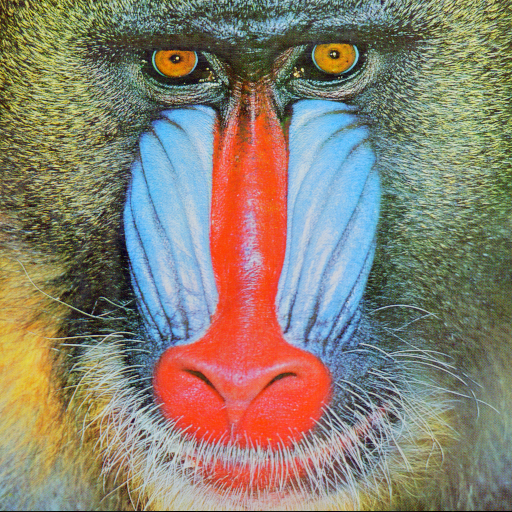
\includegraphics[scale = 0.39]{img/mandrill}
\caption{Mandrill image}
\label{mandrill}
\end{figure}

\begin{figure}[H]
\centering
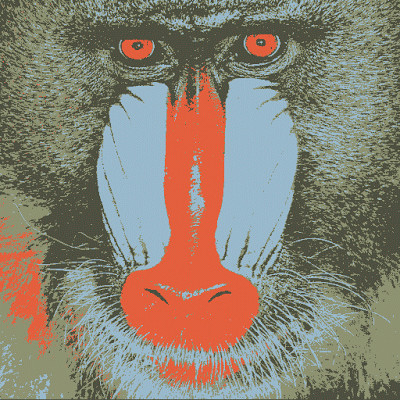
\includegraphics[scale = 0.5]{img/mandrill_segmented}
\caption{Mandrill image segmented}
\label{mandrill_segmented}
\end{figure}

\begin{figure}[H]
\centering
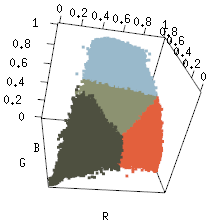
\includegraphics[scale = 0.9]{img/colormandrill-11}
\caption{Segmented mandrill image in color space}
\label{colorspacemandrill}
\end{figure}

\subsection{Image Hashing}
It is also possible to get the hash value of an image. The hash is a hexadecimal number and is another representation of the image. This is used to compare images. 

\subsubsection{Average Hashing}
The first hash method is the average hash of the image. This algorithm contains five steps.

\begin{enumerate}
        \item Convert the image to grayscale. 
        \item Reduce the size of the image, to reduce the number of computations.
        \item Average the resulting colors. For an 8x8 image, 64 will be averaged.
        \item Compute the bits of the hash value by comparing if each color value is above or below the mean.
        \item Construct the hash.
\end{enumerate}

\subsubsection{Difference Hash}
We can also compute the dHash of an image. It is similar to the average hash, but now the difference between adjacent pixels is also considered in the computation.

\subsubsection{Perceptive Hash}
This method uses the discrete cosine transform (DCT) and compares the pixels based on the frequencies, given by the DCT, instead of the color values.
DCT is a similar technique as Fourier analysis, it expresses a finite sequence of points, in this case the pixels, in terms of a sum of cosine functions.

\subsubsection{Use Of The Hash}
One application of these methods is the recognition of images. Search engines like Google use this technique to search similar images to any image you provide to the search engine.
\newline

In figure \ref{hashtable} you can see the results of applying the three types of hash to three images of a tree, figures \ref{tree1}, \ref{tree2} and \ref{tree3}. It is clear that the average hash produces similar results for every tree, while there is more difference in the results of the difference hash and the perceptive hash.

\begin{figure}[H]
\centering
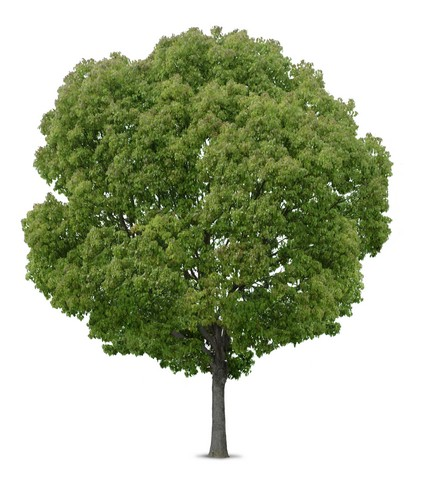
\includegraphics[scale = 1.5]{img/boom1}
\caption{Tree 1}
\label{tree1}
\end{figure}

\begin{figure}[H]
\centering
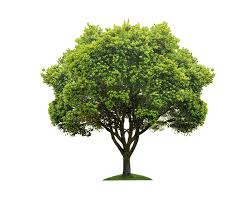
\includegraphics[]{img/boom2}
\caption{Tree 2}
\label{tree2}
\end{figure}

\begin{figure}[H]
\centering
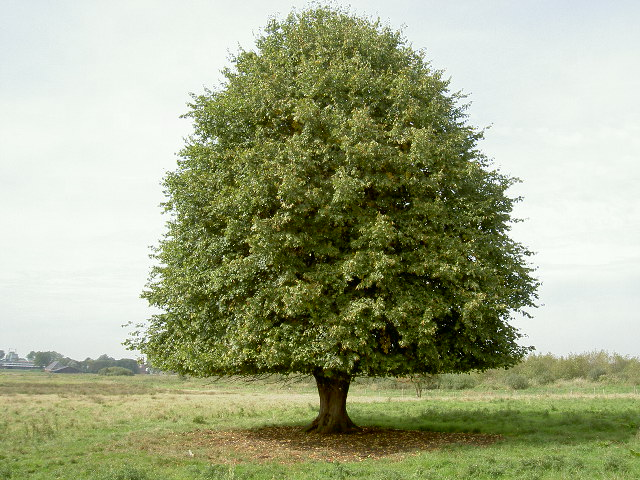
\includegraphics[scale = 0.5]{img/boom3}
\caption{Tree 3}
\label{tree3}
\end{figure}

\begin{figure}
\centering
\begin{tabular}{| c | c | c | c |}
\hline
& \textbf{Average Hash} & \textbf{Difference Hash} & \textbf{Perceptive Hash} \\
\hline
Tree 1 & ffcf8303030187ff & 00007c00b852ec7c & 7f9c2185534b98f1 \\ 
\hline
Tree 2 & ffff8f070707dfdf & 000000e804f8f800 &  4796a9695a6929d6 \\
\hline
Tree 3 & ffdf8f8787078708 & d6878788e300f8f8 & 87a569535b9899c9 \\
\hline
\end{tabular}
\caption{Table of hash results}
\label{hashtable}
\end{figure}

\subsection{Entropy}

Still another method we can use to get information from an image is to calculate the entropy.
Entropy is a measure of the amount of disorder in the image.
\newline

If all the pixels of the image have the same level of a specific parameter, the entropy is zero for that parameter. This means there is not a lot of information (almost none) to be gained from the image. An image of a blue sky has a very low entropy cause we only see blue. 
\newline

When all the pixels in the image are different, the entropy of the image is maximum and there is a lot of information to get from it. As the entropy describes how much (dis)order there is, we will eventually use this to determine how much (dis)order there is in the generated music.
\newline

To get the right entropy information about the pixels, we use a histogram that shows the count of the distinct pixel values. The entropy of an image $H$ is defined as:
\begin{equation}
H = - \sum_{k=0}^{M-1} p_k log_2 (p_k)
\end{equation}
\newline
where M is the number of unique pixel values and $p_k$ is the count of each pixel level, i.e. how many times this pixel level occurs in the image.
\newline

To illustrate the concept of entropy, I have provided two examples. In figure \ref{entropy_picasso} you can see the same painting as I used in the discussion of the edge detection algorithms. The left part of this image shows the original painting. It has quite a lot of information, there is a face with several distinguishable areas, lots of different colours and many edges. The middle part of the image shows the grayscale version of the painting. This is used to calculate the entropy [12]. The right part of the image shows the entropy for every pixel, based on the 10x10 neighbouring pixels. Red indicates a high degree of information while blue indicates a low degree.
\newline

In figure \ref{entropy_blue_red} you can see the results of the algorithm applied to an image with very little information. The left part of the image shows the original image, which is a blue and red image. The middle part again shows the grayscale version of the original. The right part again shows the entropy for every pixel. As expected, we only have a high degree of information on the edge between the blue and the red parts.
  
\begin{figure}[H]
\hspace*{-0.8cm}
\centering
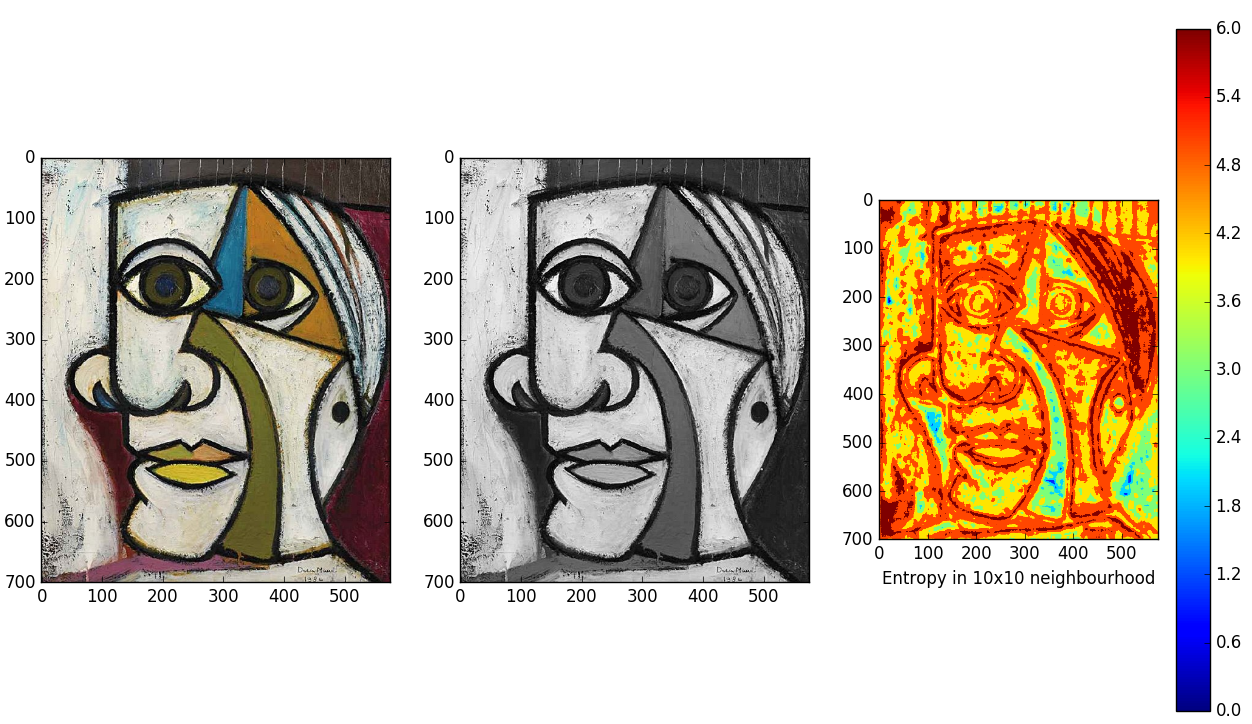
\includegraphics[scale = 0.35]{img/entropy_picasso}
\caption{Entropy of the Picasso, figure \ref{picasso}}
\label{entropy_picasso}
\end{figure} 

\begin{figure}[H]
\centering
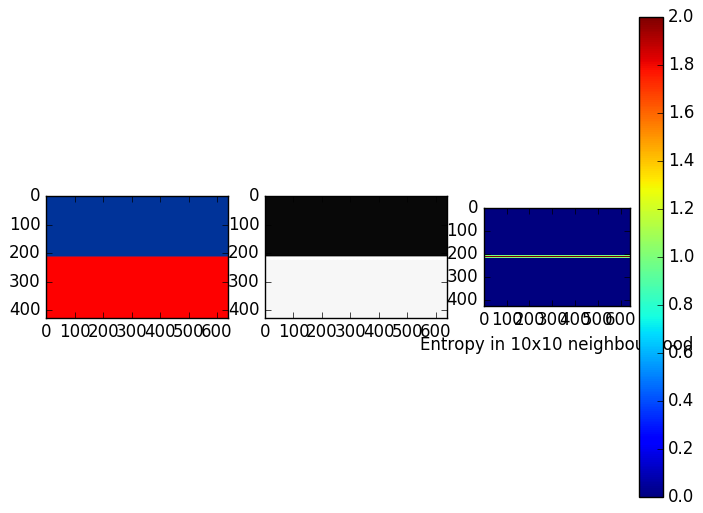
\includegraphics[scale = 0.54]{img/entropy_blue_red}
\caption{Entropy of a blue and red image}
\label{entropy_blue_red}
\end{figure} 
\newpage

\section{Text Processing Algorithms}

To conclude this paper, I will discuss text processing algorithms because it can be a nice addition to the purely graphical algorithms discussed so far. 
In text processing, text in an image is recognized and its meaning extracted. Eventually we could use this information for sentiment analysis.

\subsection{Pre-processing}

Text processing starts with recognizing the individual characters, this is called Optical Character Recognization (OCR). To increase the effectiveness of the OCR algorithms we can pre-process the images.
Several techniques can be used.

\paragraph{Layout analysis}

Often called 'zoning', this technique identifies columns, paragraphs, sections, etc as distinct blocks.

\paragraph{Character isolation}

If you want to apply OCR to every character separately (per-character OCR), this technique breaks groups of multiple characters into single letters.

\paragraph{Binarisation}

Converts the image from color to grayscale. It is a simple way to separate the text from the background of the image. Most OCR algorithms work only on grayscale images since these images are easier to work with. 

\subsection{Character Recognition}

\subsubsection{Pattern Recognition}

One of the first techniques developed is pattern recognition, sometimes called matrix matching. This technique involves comparing an image of text to a previously stored glyph\footnote{A matrix representation of the symbol, intended to represent a readable character.} on a pixel-by-pixel basis. This only works if the glyph and the input text are in the same font, same scale and if the input text can be isolated from the rest of the image.
\newline

This is very similar to classification in supervised machine learning . We have some learning data (the stored glyph) and we use this to get the correct results from unknown data.

\subsubsection{Feature Extraction}

This techinque uses 'features' as glyphs, for example, lines, closed loops and line intersection. Using these features instead of the complete glyph reduces dimensionality and makes the recognition computationally more efficient.
\newline

An example of an algorithm used is the k-nearest neighbour classification algorithm or $k$-NN. It is used to compare image features with stored glyph features and chooses the nearest match. Labeled training data is needed, since it is a supervised learning algorithm. Important to notice is that the feature vectors are in a multidimensional feature space, each with a class label. Storing the vectors in a multidimensional space allows us to calculate the distances between vectors. This distance will be used to choose the best classification. A new instance (in this case a character to recognise) is classified by assigning the label of the feature vector which is most frequent among the $k$ training samples nearest to the test sample [16]. 
\newline

The Euclidian distance is commonly used to determine the distance between two continous samples. If the variables are discrete, which is the case in text classification, the overlap metric or Hamming distance is used. This metric is the number of positions at which the symbols to compare are different. In figure \ref{hamming} you can see an example of this metric. The distance between $100$ and $011$ is $3$, which is the number of sides of the cube you have to follow to get from $100$ to $011$ [17].
\newline

In figure \ref{kNN} you can see an example of the $k$-NN algorithm. The green circle is the new instance. To determine if it should be classified as a blue square or as a red triangle, we look at the number of occurences of the possible classifications in the circle. The solid line circle is the space created by the algorithm with $k = 3$. Now the green circle is seen as a red triangle, because there are two red triangles and only one blue square. If $k = 5$, the space created by k-NN is the dashed line circle. Now the algorithm would classify the green circle as a blue square because there are two red triangles and three blue squares in the circle. 

\begin{figure}[H]
\centering
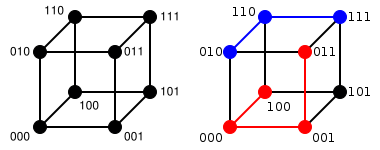
\includegraphics[scale = 0.65]{img/hamming}
\caption{Example of the Hamming metric}
\label{hamming}
\end{figure} 

\begin{figure}[H]
\centering
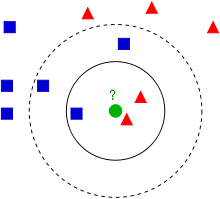
\includegraphics[scale = 0.6]{img/kNN}
\caption{Example of the $k$-NN algorithm}
\label{kNN}
\end{figure} 
\newpage

\section{Conclusion}

Eventually the ArtToMusic application will extract useful data from all the algorithms discussed in this paper. In this section I will run several algorithms on several paintings, each in a completely different style. At the end we will have a collection of parameters we can use to generate music. I will use the painting of Picasso, figure \ref{picasso}, a painting of Bruegel, figure \ref{bruegel} and a painting of Mondriaan, figure \ref{mondriaan}.
\newline

These three paintings are very different. The Bruegel is very busy and intricate, so we expect results that represent this, for example a high entropy of the edge detection result. The Picasso is a face so it's not a busy painting, but with a wide range of colours we expect a high value for $k$ in the image segmentation algorithm. The Mondriaan, figure \ref{mondriaan} consists of big squares of solid colours which suggets a low amount of edges and a low entropy in general.

\subsection{Picasso}

\subsubsection{Noise Removal}

As discussed in section 2.3 we have four noise removal ralgorithms. To use these algorithms in a meaningfull way, we can apply one of them on the image before the edge detection step to improve the results of the edge detection algorithm. In order for the noise removal algorithms to work we first have to convert the images to gray scale images.
\newline

In figure \ref{noise_picasso} you can see the results of the four algorithms. The median filter gives us the clearest result, as expected cause this is the most statistical robust filter of the four discussed here. Since the Gaussian filter also smooths the image, we won't be using this to detect the edges, even though the noise is removed. The median and the rank filter are not adequate enough to compete with the other filters.

\begin{figure}[H]
\hspace*{-0.70cm}
\centering
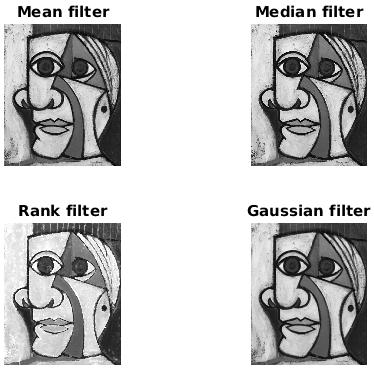
\includegraphics[scale = 0.85]{img/picasso_noise}
\caption{Results of noise removal algorithms on the Picasso}
\label{noise_picasso}
\end{figure} 

\subsubsection{Edge Detection}

Let's look at the results of the edge detection algorithms for the Picasso. The resulting images can be found in section 2.1. We want to get as much information as possible from the result of the edge detection. When we look at the entropy of each resulting image, it is clear that the results of the algorithms are very close to each other. In table \ref{entropy_results} you can see the entropies of the columns of each resulting image. In this case we will choose the algorithm with the highest entropy, the LoG algorithm. The resulting output image is figure \ref{log}.
\newline

\begin{figure}[H]
\hspace*{-0.70cm}
\begin{tabular}{| c | c | c | c | c | c | c |}
\hline
& \textbf{Sobel} & \textbf{Frei Chen} & \textbf{Prewitt} & \textbf{Roberts Cross} & \textbf{LoG} & \textbf{Scharr} \\
\hline
Entropy & 12.30425 & 12.30326 & 12.30373 & 12.32597 & 12.88781 & 12.30777 \\ 
\hline
\end{tabular}
\caption{Entropies of edge detection algorithms on the Picasso}
\label{entropy_results}
\end{figure} 

The output from this algorithm is a matrix representing the edges of the image. We need to get information about this matrix to create useful input parameters. For instance, we can count the number of distinct values in the matrix. This gives us an idea of how many edges there are. When we round the pixel values of the output of the edge detection algorithm to three decimals we get a good value. Less than three decimals doesn't show the difference between the paintings and more than three decimals returns a number that almost represents the whole matrix. For the LoG algorithm this gives us 811 unique values. To translate this into an input parameter we can create a scale, ranging from 500 to 1500\footnote{This is an arbitrary chosen scale.} and see where the calculated number is situated on this scale. A low number of edges can result in a slow piece of music and a high number of edges can result in a fast piece of music.

\subsubsection{Image Segmentation}

Using the technique of image segmentation we can get the amount of colors in the image. Analogous to the results of the edge detection we can create a scale that represents the possible values of $k$. A low $k$ (e.g. 1 or 2) will result in a piece of music with very few notes, while a high $k$ (e.g. 20 and upwards) will result in a busy piece of music. If we run this algorithm on the same Picasso of figure \ref{picasso} we get the following result. When we use $k = 15$ we get a satisfying result. Figure \ref{picasso_segmented} shows the segmented Picasso painting and figure \ref{picasso_colors} shows the colors in the RGB color space. The segmented image is very close to the original image cause we were able to find sufficient colours to reconstruct the image.

\begin{figure}[h]
\hspace*{-0.70cm}
\centering
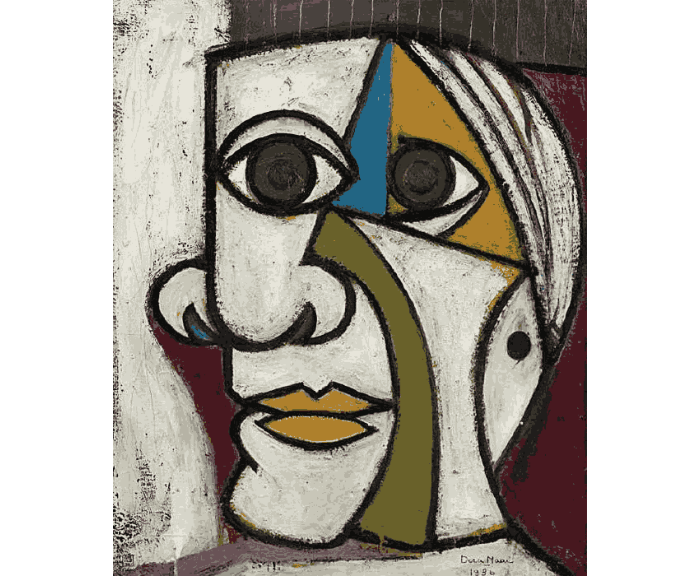
\includegraphics[scale = 0.5]{img/picasso_segmented}
\caption{The Picasso segmented in colours}
\label{picasso_segmented}
\end{figure} 

\begin{figure}[h]
\centering
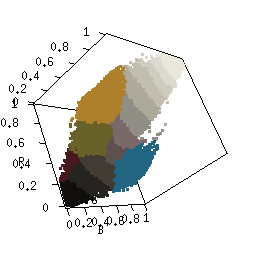
\includegraphics[scale = 0.9]{img/picasso_colors}
\caption{Colours of the Picasso}
\label{picasso_colors}
\end{figure}

\subsubsection{Colours}

The image segmentation not only returns the number of colours (clusters) in the painting, it also specifies what these colours are. In the table below you can see the 15 colours extracted from the Picasso painting, shown in figure \ref{picasso_colors}. You can see the RGB value of each colour, in 255 format and in percentage, as well as the HSV value. The hexadecimal representation is also included.

\begin{tabular}{| c | c | c | c | c | c | c |}
\hline
\textbf{Hex} & \textbf{R} & \textbf{G} & \textbf{B} & \textbf{H} & \textbf{S} & \textbf{V} \\
\hline
\#0D0D0A & 13 (5\%) & 13 (5\%) & 10 (4\%) &  60° & 23\% & 5\% \\ 
\hline
\#695757 & 105 (41\%) & 87 (34\%) & 87 (34\%) & 0° & 17\% & 41\% \\ 
\hline
\#B5B3A6 & 181 (71\%) & 179 (70\%) & 166 (65\%) & 52° & 8\% & 71\% \\ 
\hline
\#D6D4C9 & 214 (84\%) & 212 (83\%) & 201 (79\%) & 52° & 6\% & 84\% \\ 
\hline
\#C7C7B8 & 199 (78\%) & 199 (78\%) & 184 (72\%) & 60° & 8\% & 78\% \\ 
\hline
\#E6E6DB & 230 (90\%) & 230 (90\%) & 219 (86\%) & 60° & 5\% & 90\% \\ 
\hline
 \#7D756E & 125 (49\%) & 117 (46\%) & 110 (43\%) & 28° & 12\% & 49\% \\ 
\hline
\#363029 & 54 (21\%) & 48 (19\%) & 41 (16\%) & 32° & 24\% & 21\% \\ 
\hline
\#AD802B & 173 (68\%) & 128 (50\%) & 43 (17\%) & 39° & 75\% & 68\% \\ 
\hline
\#696129 & 105 (41\%) & 97 (38\%) & 41 (16\%) & 52° & 61\% & 41\% \\ 
\hline
\#471A1F & 71 (28\%) & 26 (10\%) & 31 (12\%) & 354° & 63\% & 28\% \\ 
\hline
\#216682 & 33 (13\%) & 102 (40\%) & 130 (51\%) & 198° & 75\% & 51\% \\ 
\hline
\#AB998A & 171 (67\%) & 153 (60\%) & 138 (54\%) & 28° & 19\% & 67\% \\ 
\hline
\#1F1F1A & 31 (12\%) & 31 (12\%) & 26 (10\%) & 60° & 16\% & 12\% \\ 
\hline
\#4A423D & 74 (29\%) & 66 (26\%) & 61 (24\%) & 24° & 18\% & 29\% \\ 
\hline
\end{tabular}

\subsection{Bruegel}

As explained above, we use a painting of Bruegel, figure \ref{bruegel}, because we expect results from the algorithms that indicate a busy, high tempo piece of music.

\begin{figure}[h]
\hspace*{-0.70cm}
\centering
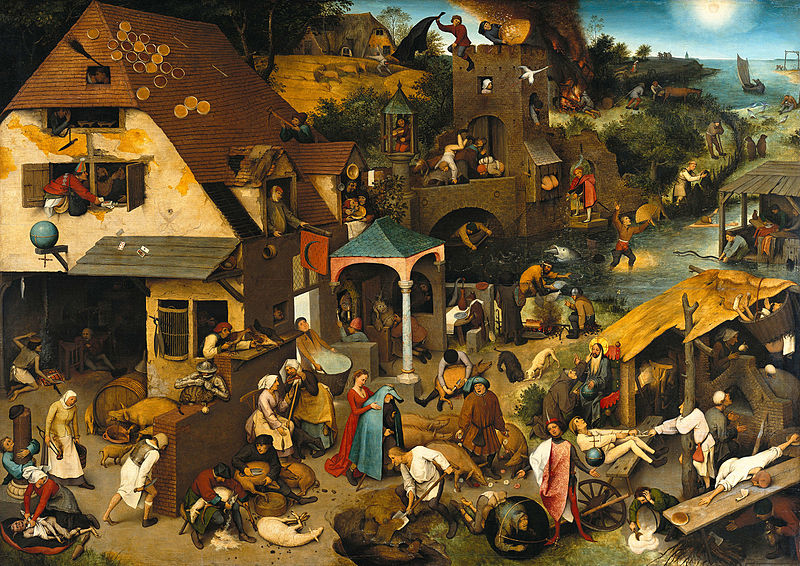
\includegraphics[scale = 0.4]{img/bruegel}
\caption{The Bruegel}
\label{bruegel}
\end{figure} 

\subsubsection{Noise Removal}

When we apply the four noise removal algorithms to the Bruegel we get the result in figure \ref{noise_bruegel}.
We can draw the same conclusion as with the Picasso. The median filter the best to work with. Gaussian filter is a close second, but the smoothing of the image causes us the disregard it, thinking of the edge detection algorithms. 

\begin{figure}[H]
\hspace*{-0.70cm}
\centering
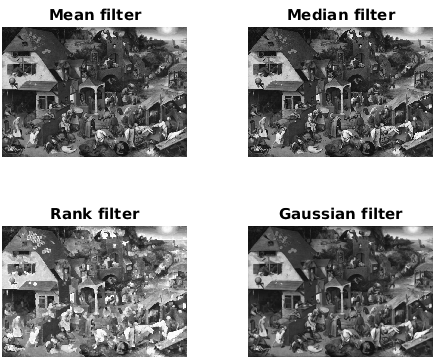
\includegraphics[scale = 1]{img/bruegel_noise}
\caption{Results of noise removal algorithms on the Bruegel}
\label{noise_bruegel}
\end{figure}

\subsubsection{Edge Detection}

Analogous to the Picasso, I applied the six edge detection algorithms to the Bruegel painting. In table \ref{bruegel_entropy} you can see the results. As with the Picasso, the LoG algorithm has the highest entropy. We find 848 unique values, so this would give a similar tempo as the Picasso.

\begin{figure}
\begin{tabular}{| c | c | c | c | c | c | c |}
\hline
& \textbf{Sobel} & \textbf{Frei Chen} & \textbf{Prewitt} & \textbf{Roberts Cross} & \textbf{LoG} & \textbf{Scharr} \\
\hline
Entropy & 12.56623 & 12.56724 & 12.57051 & 12.59074 & 13.01124 & 12.5687 \\ 
\hline
\end{tabular}
\caption{Entropies of edge detection algorithms on the Bruegel}
\label{bruegel_entropy}
\end{figure} 
\newpage
\subsubsection{Image Segmentation}

When we apply the image segmentation algorithm to the painting of Bruegel, we can see that it takes $k = 20$ clusters to classify enough colours. This is a big number, more than we needed with the Picasso, so we expect a busy piece of music to be generated based on this parameter. In figure \ref{bruegel_segmented} you can see the segmented version of this painting. Since our $k$ is so high, there is not so much difference between the original painting and this version. In figure \ref{bruegel_colors} you can see the colours extracted.  

\begin{figure}[h]
\hspace*{-0.70cm}
\centering
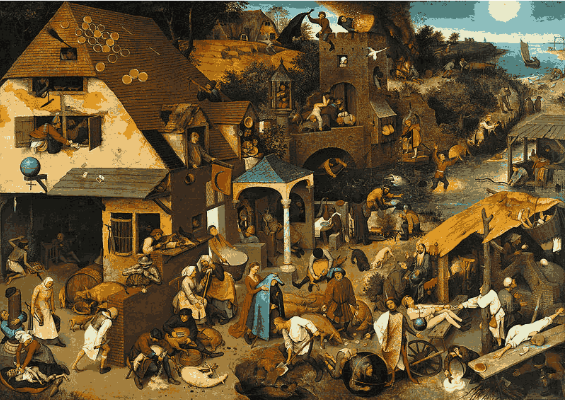
\includegraphics[scale = 0.55]{img/bruegel_segmented}
\caption{The Bruegel segmented in colours}
\label{bruegel_segmented}
\end{figure} 

\begin{figure}[H]
\centering
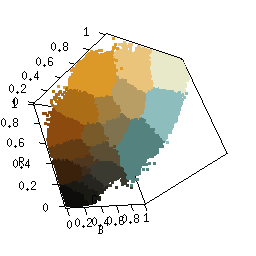
\includegraphics[scale = 0.8]{img/bruegel_colors}
\caption{Colours of the Bruegel}
\label{bruegel_colors}
\end{figure}
\newpage

\subsubsection{Colours}

Analogous to the Picasso painting, below are the 20 colours of the Bruegel painting.
\newline

\begin{tabular}{| c | c | c | c | c | c | c |}
\hline
\textbf{Hex} & \textbf{R} & \textbf{G} & \textbf{B} & \textbf{H} & \textbf{S} & \textbf{V} \\
\hline
\#B17817 & 177 (69\%) & 120 (44\%) & 23 (9\%) & 38° & 87\% & 69\% \\ 
\hline
\#E3AD57 & 227 (89\%) & 173 (68\%) & 87 (34\%) & 37° & 62\% & 89\% \\ 
\hline
\#B3A173 & 179 (70\%) & 161 (63\%) & 115 (45\%) & 44° & 36\% & 70\% \\ 
\hline
\#A88542 & 168 (66\%) & 133 (52\%) & 66 (26\%) & 40° & 61\% & 66\% \\ 
\hline
\#695733 & 105 (41\%) & 87 (34\%) & 51 (20\%) & 40° & 51\% & 41\% \\ 
\hline
\#47736B & 71 (28\%) & 115 (45\%) & 107 (42\%) & 170° & 38\% & 45\% \\ 
\hline
\#DB961C & 219 (86\%) & 150 (59\%) & 28 (11\%) & 38° & 87\% & 86\% \\ 
\hline
\#4D402E & 77 (30\%) & 64 (25\%) & 46 (18\%) & 36° & 40\% & 30\% \\ 
\hline
\#241F1A & 36 (14\%) & 31 (12\%) & 26 (10\%) & 30° & 28\% & 14\% \\ 
\hline
\#4A2E14 & 74 (29\%) & 46 (18\%) & 20 (8\%) & 29° & 73\% & 29\% \\ 
\hline
\#12120F & 18 (7\%) & 18 (7\%) & 15 (6\%) & 60° & 17\% & 7\% \\ 
\hline
\#8C4D12 & 140 (55\%) & 77 (30\%) & 18 (7\%) & 30° & 87\% & 55\% \\ 
\hline
\#F7F7C7 & 247 (95\%) & 247 (97\%) & 199 (78\%) & 60° & 19\% & 97\% \\ 
\hline
\#362E24 & 54 (21\%) & 46 (18\%) & 36 (14\%) & 34° & 33\% & 21\% \\ 
\hline
\#6BA1A1 & 107 (42\%) & 161 (63\%) & 161 (63\%) & 180° & 34\% & 63\% \\ 
\hline
\#876930 & 135 (53\%) & 105 (41\%) & 48 (19\%) & 40° & 64\% & 53\% \\ 
\hline
\#A6D1CF & 166 (65\%) & 209 (82\%) & 207 (81\%) & 72° & 100\% & 82\% \\ 
\hline
\#EDCC85 & 237 (93\%) & 204 (80\%) & 133 (52\%) & 42° & 44\% & 93\% \\ 
\hline
\#827857 & 130 (51\%) & 120 (47\%) & 87 (34\%) & 46° & 33\% & 51\% \\ 
\hline
\#664017 & 102 (40\%) & 64 (25\%) & 23 (9\%) & 32° & 77\% & 40\% \\ 
\hline
\end{tabular}

\newpage
\subsection{Mondriaan}

To conlude the comparison, a painting of Mondriaan is used, figure \ref{mondriaan}. Mondriaan's paintings were famous for its straight lines and full colours. We expect results that indicate a piece of music with little notes and not so difficult or busy rhythms.

\begin{figure}[H]
\centering
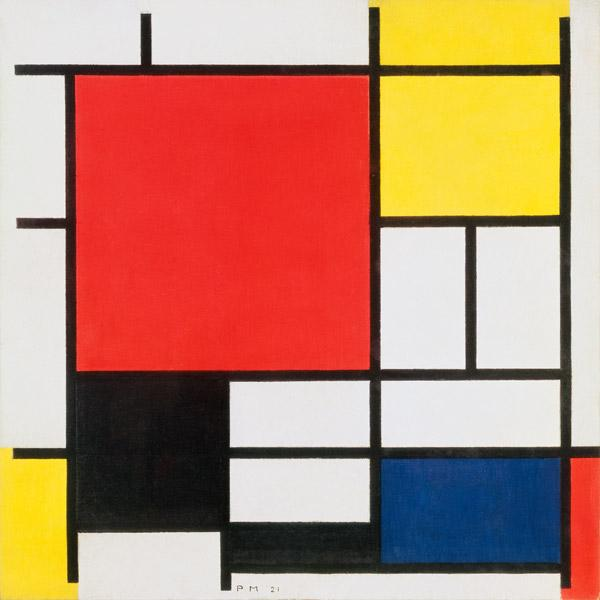
\includegraphics[scale = 0.6]{img/mondriaan}
\caption{The Mondriaan}
\label{mondriaan}
\end{figure}

\subsubsection{Noise Removal}

When we apply the four noise removal algorithms to the Mondriaan we get the result in figure \ref{noise_mondriaan}.
Since there are a lot of squares of full colour and not so many edges in this image, the results of the noise removal algorithms are very similar. To continue the trend we again choose the median filter to work with.

\begin{figure}[H]
\centering
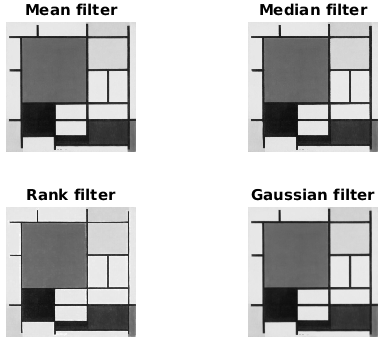
\includegraphics[scale = 1]{img/mondriaan_noise}
\caption{Results of noise removal algorithms on the Mondriaan}
\label{noise_mondriaan}
\end{figure}

\subsubsection{Edge Detection}

Analogous to the Picasso and the Bruegel, the six edge detection algorithms were applied to the Mondriaan painting. In table \ref{mondriaan_entropy} you can see the results. As with the Picasso and the Bruegel, the LoG algorithm has the highest entropy. We find 806 unique values, so this would again give a similar tempo as the Picasso and the Bruegel. This result is unexpected because with the naked eye we see very little edges on the Mondriaan painting and would expect a lower number of unique values than the two previous paintings. The overall entropy is lower in this painting, which was to be expected, but the difference between the entropies of the Mondriaan and the Picasso is less than expected.

\begin{figure}[H]
\hspace*{-0.70cm}
\begin{tabular}{| c | c | c | c | c | c | c |}
\hline
& \textbf{Sobel} & \textbf{Frei Chen} & \textbf{Prewitt} & \textbf{Roberts Cross} & \textbf{LoG} & \textbf{Scharr} \\
\hline
Entropy & 11.0401 & 11.03431 & 11.03016 & 11.02275 & 12.77017 & 11.05094 \\ 
\hline
\end{tabular}
\caption{Entropies of edge detection algorithms on the Mondriaan}
\label{mondriaan_entropy}
\end{figure} 

\subsubsection{Image Segmentation}

When we apply the image segmentation algorithm to the painting of Mondriaan, we can see that it takes $k = 6$ clusters. Since it is a small number, our expectations of a simple piece of music are confirmed (for now). In figure \ref{mondriaan_segmented} you can see the segmented version of this painting. Even though we have a low $k$, we don't see any difference between the original and the segmented version. This is because the original was already very segmented, all the colours are separated from each other by black lines. This makes it easier to segment it and results in less colours. In figure \ref{mondriaan_colors} you can see the colours extracted.  

\begin{figure}[H]
\centering
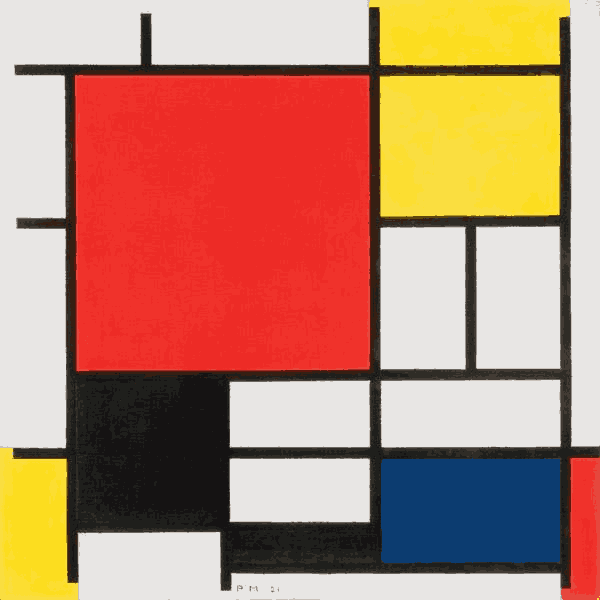
\includegraphics[scale = 0.4]{img/mondriaan_segmented}
\caption{The Mondriaan segmented in colours}
\label{mondriaan_segmented}
\end{figure}

\begin{figure}[H]
\centering
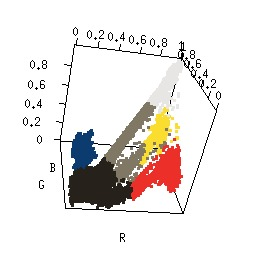
\includegraphics[scale = 0.7]{img/mondriaan_colors}
\caption{Colours of the Mondriaan}
\label{mondriaan_colors}
\end{figure}

\subsubsection{Colours}

Below are the colours of the Mondriaan painting.
\newline

\begin{tabular}{| c | c | c | c | c | c | c |}
\hline
\textbf{Hex} & \textbf{R} & \textbf{G} & \textbf{B} & \textbf{H} & \textbf{S} & \textbf{V} \\
\hline
\#FCDE30 & 252 (99\%) & 222 (87\%) & 48 (19\%) & 52° & 81\% & 99\% \\ 
\hline
\#E6E6E3 & 230 (90\%) & 230 (90\%) & 227 (89\%) & 60° & 1\% & 90\% \\ 
\hline
\#26211C & 38 (15\%) & 38 13(\%) & 28 (11\%) & 30° & 26\% & 15\% \\ 
\hline
\#ED2E29 & 237 (93\%) & 46 (18\%) & 41 (16\%) & 2° & 83\% & 93\% \\ 
\hline
\#807863 & 128 (50\%) & 120 (47\%) & 99 (39\%) & 44° & 23\% & 50\% \\ 
\hline
\#143B70 & 20 (8\%) & 59 (23\%) & 112 (44\%) & 216° & 82\% & 44\% \\ 
\hline
\end{tabular}

\newpage

\begin{thebibliography}{1}

\bibitem{OpenImageR} Lampros Mouselimis {\em OpenPackageR, An Image Processing Toolkit} 2017

\bibitem{Convolution} R. Fisher, S. Perkins, A. Walker, E. Wolfart {\em Hypermedia Image Processing Reference} 2003

\bibitem{Frei_Chen_Sobel} Daniel R\'akos' blog (\url{http://rastergrid.com/blog/2011/01/frei-chen-edge-detector/}) 2011

\bibitem{Gaussian} University of Auckland, New Zealand, Computer Science course Computer Graphics and Image Processing {\em Gaussian Filtering} 2010

\bibitem{edge} Computaç\~ao Visual e Multimédia, course on Image Processing

\bibitem{prewitt} RoboRealm blog (\url{http://www.roborealm.com/help/Prewitt.php}) 2017

\bibitem{scharr} Jogn Costella's blog ( \url{http://johncostella.com/edgedetect/}) 2012

\bibitem{image filter} Simon Colton, Pedro Torres {\em Evolving Approximate Image Filters} 2009, Computational Creativity Group
Department of Computing, Imperial College London

\bibitem{hash} Dr. Neal Krawetz' blog (\url{http://www.hackerfactor.com/blog/?/archives/529-Kind-of-Like-That.html}) 2013

\bibitem{entropy} John Loomis' site (\url{http://www.johnloomis.org/ece563/notes/basics/entropy/entropy.html}) 1998

\bibitem{entropy} Kevin Meurer's blog (\url{http://kevinmeurer.com/a-simple-guide-to-entropy-based-discretization/}) 2015

\bibitem{entropy_python} Python Multimedia Codec Exercices Documentation (\url{https://www.hdm-stuttgart.de/~maucher/Python/MMCodecs/html/basicFunctions.html}) 2013

\bibitem{color} Ryan Walker's blogpost (\url{https://www.r-bloggers.com/color-quantization-in-r/}) 2016

\bibitem{noise} C. Solomon, T. Breckon {\em Fundamentals of Digital Image Processing: A Practical Approach with Examples in Matlab} 2011

\bibitem{OCR} \url{https://en.wikipedia.org/wiki/Optical_character_recognition}

\bibitem{kNN} \url{https://en.wikipedia.org/wiki/K-nearest_neighbors_algorithm}

\bibitem{hamming} \url{https://en.wikipedia.org/wiki/Hamming_distance}
\end{thebibliography}

\end{document}
